% ResearchX literature review — academic report style.
% Layout reference: proposal.pdf (Times text, A4, roman front matter, numbered chapters).
% Build: xelatex literature-review.tex (twice, for TOC/LOF/LOT).
\documentclass[12pt,a4paper]{report}

\usepackage{fontspec}
\setmainfont{Times New Roman}
\usepackage{amsmath,amssymb}
\numberwithin{equation}{chapter}
\usepackage{geometry}
\geometry{a4paper,margin=1in}
\usepackage{setspace}
\onehalfspacing
\usepackage{titlesec}
\renewcommand{\chaptername}{CHAPTER}
\titleformat{\chapter}[display]{\normalfont\bfseries\centering}{\chaptername\ \thechapter}{12pt}{\large}
\titlespacing*{\chapter}{0pt}{-20pt}{20pt}
\titleformat{\section}{\normalfont\bfseries}{\thesection}{1em}{}
\titleformat{\subsection}{\normalfont\bfseries}{\thesubsection}{1em}{}
\usepackage{graphicx}
\usepackage{booktabs}
\usepackage{array}
\usepackage[table]{xcolor}
\usepackage{tikz}
\usetikzlibrary{positioning,fit,arrows.meta}
\usepackage[hidelinks]{hyperref}
\setlength{\tabcolsep}{4pt}
\renewcommand{\arraystretch}{1.15}
\newcolumntype{L}[1]{>{\raggedright\arraybackslash}p{#1}}

\begin{document}

% ---------------- Title page ----------------
\begin{titlepage}
\begin{center}
{\large FUSEMACHINE PROJECT\par}
\vspace{1.0cm}
{\Large\bfseries ResearchX: An Autonomous AI Agent Harness\\for Research and Paper Writing\par}
\vspace{0.5cm}
{\large A Literature Review and Implementation Audit\par}
\vspace{1.0cm}
{\large PREPARED BY\par}
\vspace{0.3cm}
{\large Chandan Shah\par}
{\large Viraj Sawad\par}
{\large Janvi Rajbhandari\par}
\vspace{1.0cm}
{\large PREPARED FOR THE FUSEMACHINE PROJECT\par}
\vspace{0.5cm}
{\large SEPTEMBER, 2026\par}
\end{center}
\end{titlepage}

% ---------------- Front matter ----------------
\pagenumbering{roman}

\chapter*{ABSTRACT}
\addcontentsline{toc}{chapter}{ABSTRACT}
Research does not fail for lack of papers alone. It fails when discovery,
execution, verification and writing are disconnected. This review examines
ResearchX as a proposed terminal (TUI) research agent: a question enters, the
system assembles source-backed evidence and experiment artifacts, and a human
must approve any final draft. Chapter~2 states the problem and six acceptance
criteria. Chapter~3 reviews the Pi harness, related research agents and
research-writing products, and the open discovery sources. Chapter~4 records
the previously discussed architecture and the design corrections. Chapter~5
constructs a comparative capability pipeline. Chapter~6 documents the source
stack and the current verification limitation. Chapter~7 gives the proposed
ResearchX design and audits its implementation status.

The audit is deliberately conservative. Pi-native integration, PaperRank,
science-database search, Kaggle tools, the skeptic workflow and the persisted
human checkpoint are present in the checked-out source tree. The citation
verifier still calls Semantic Scholar, and a dedicated hypothesis-branch,
append-only findings-ledger and doom-loop implementation is not yet evidenced
as a completed ResearchX feature. Those gaps are recorded instead of being
presented as shipped capabilities.

\tableofcontents
\addcontentsline{toc}{chapter}{TABLE OF CONTENTS}
\listoffigures
\addcontentsline{toc}{chapter}{LIST OF FIGURES}
\listoftables
\addcontentsline{toc}{chapter}{LIST OF TABLES}

\chapter*{ABBREVIATIONS}
\addcontentsline{toc}{chapter}{ABBREVIATIONS}
\begin{tabular}{@{}ll@{}}
API & Application Programming Interface \\
ARS & Academic Research Skills (stage-gate methodology reference) \\
CLI & Command-Line Interface \\
DOI & Digital Object Identifier \\
GPU & Graphics Processing Unit \\
OA  & Open Access \\
Pi  & Base agent harness runtime of ResearchX \\
S2  & Semantic Scholar (current verifier dependency under review) \\
SOTA & State of the Art \\
TUI & Terminal User Interface \\
\end{tabular}
\clearpage
\pagenumbering{arabic}

% ---------------- Chapter 1 ----------------
\chapter{INTRODUCTION}

ResearchX is being developed as a terminal (TUI) research agent with a
verifiable-output contract: a research question should produce source-backed
evidence and a draft that is not final until a human approves it. The discussed
architecture has four layers over a foundation. The Research layer searches,
ranks and synthesises papers and audits code against paper claims. The
Experiment layer is intended to isolate hypotheses, record runs and stop
repeated failures. The Integrity layer is intended to verify citations, link
empirical claims to logged results and enforce a human checkpoint. The Writing
layer drafts from verified findings and applies a skeptic review pass. The
foundation provides the agent orchestrator, tool manager, memory, prompt and
context management, and logging with monitoring.

The intended data flow is Inputs to Research to Experiment to Integrity to
Writing to Human Approval, with paper sources attached to Research, compute
attached to Experiment, and verification sources attached to Integrity.
Figure~1.1 redraws that contract on the actual runtime boundary.

The base claim of this review is that the base harness is the Pi agent
harness~\cite{pi}. Pi owns the interactive agent loop and the native TUI,
model and provider routing, tool and extension registration with a session-start
lifecycle, and sessions with researcher, reviewer, writer and verifier
subagents. Other research systems are treated as feature references only; none
of them is the base runtime.

\begin{figure}[ht]
\centering
\resizebox{\textwidth}{!}{%
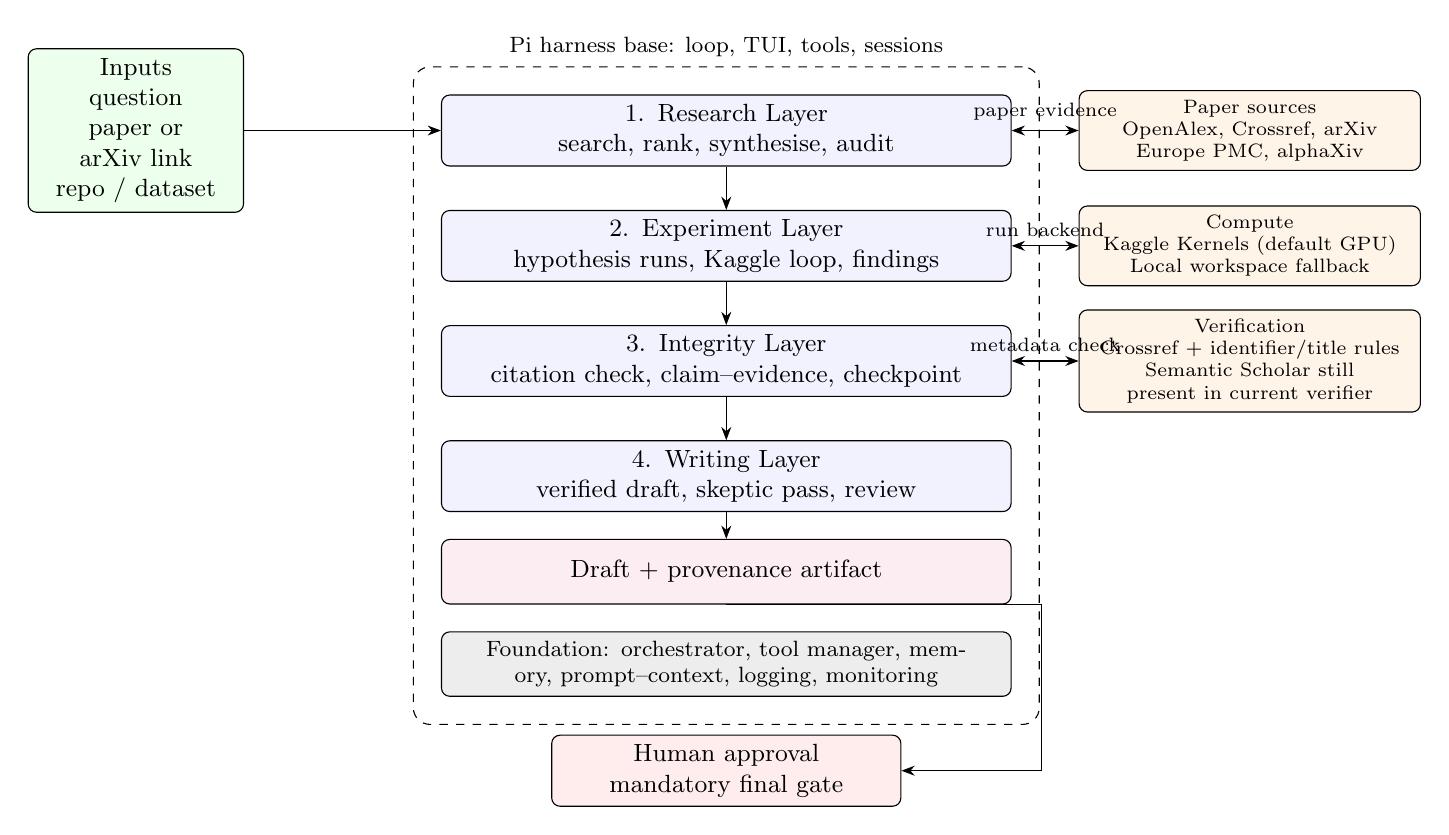
\begin{tikzpicture}[
  font=\small,
  layer/.style={draw, rounded corners=3pt, fill=blue!5, align=center,
    text width=7.0cm, minimum height=0.82cm},
  input/.style={draw, rounded corners=3pt, fill=green!7, align=center,
    text width=2.5cm, minimum height=1.15cm},
  service/.style={draw, rounded corners=3pt, fill=orange!9, align=center,
    text width=4.1cm, minimum height=1.0cm, font=\scriptsize},
  artifact/.style={draw, rounded corners=3pt, fill=purple!7, align=center,
    text width=7.0cm, minimum height=0.82cm},
  foundation/.style={draw, rounded corners=3pt, fill=gray!14, align=center,
    text width=7.0cm, minimum height=0.72cm, font=\footnotesize},
  gate/.style={draw, rounded corners=3pt, fill=red!7, align=center,
    text width=4.2cm, minimum height=0.82cm},
  base/.style={draw, dashed, rounded corners=6pt, inner sep=0.35cm},
  >=Stealth
]
\node[layer] (rl) {1. Research Layer\\search, rank, synthesise, audit};
\node[layer, below=0.55cm of rl] (el) {2. Experiment Layer\\hypothesis runs, Kaggle loop, findings};
\node[layer, below=0.55cm of el] (il) {3. Integrity Layer\\citation check, claim--evidence, checkpoint};
\node[layer, below=0.55cm of il] (wl) {4. Writing Layer\\verified draft, skeptic pass, review};
\node[input, left=2.5cm of rl] (inp) {Inputs\\question\\paper or arXiv link\\repo / dataset};
\node[service, right=0.85cm of rl] (src) {Paper sources\\OpenAlex, Crossref, arXiv\\Europe PMC, alphaXiv};
\node[service, right=0.85cm of el] (cmp) {Compute\\Kaggle Kernels (default GPU)\\Local workspace fallback};
\node[service, right=0.85cm of il] (ver) {Verification\\Crossref + identifier/title rules\\Semantic Scholar still present in current verifier};
\node[artifact, below=0.34cm of wl] (out) {Draft + provenance artifact};
\node[foundation, below=0.34cm of out] (fnd) {Foundation: orchestrator, tool manager, memory, prompt--context, logging, monitoring};
\node[gate, below=0.48cm of fnd] (gate) {Human approval\\mandatory final gate};
\node[base, fit=(rl) (el) (il) (wl) (out) (fnd), label={[font=\footnotesize]above:Pi harness base: loop, TUI, tools, sessions}] (pi) {};
\draw[->] (inp) -- (rl);
\draw[->] (rl) -- (el);
\draw[->] (el) -- (il);
\draw[->] (il) -- (wl);
\draw[->] (wl) -- (out);
\draw[->] (out.south) -- ++(4.0cm,0) |- (gate.east);
\draw[<->] (rl) -- node[above, font=\scriptsize] {paper evidence} (src);
\draw[<->] (el) -- node[above, font=\scriptsize] {run backend} (cmp);
\draw[<->] (il) -- node[above, font=\scriptsize] {metadata check} (ver);
\end{tikzpicture}%
}
\caption{ResearchX four-layer architecture on the Pi harness base. Solid arrows
show the evidence flow; the double-headed links attach paper sources, compute
and verification to their relevant layer. The human approval gate remains
outside the Pi-owned runtime.}
\end{figure}

% ---------------- Chapter 2 ----------------
\chapter{PROBLEM STATEMENT}

\section{Context}
Research tooling creates a separation problem. Search systems return many
papers but do not by themselves establish whether a paper supports the claim
being written. Writing assistants can attach useful citations without proving
that the cited metadata or interpretation is correct. Notebook and experiment
systems can execute code while leaving source selection, claim tracing and
review approval to the user. These are useful capabilities, but they do not
automatically form one auditable research record.

\section{Problem Formulation}
Let a research question $q$ and a corpus of candidate papers $D$ be given. A
research agent must produce a draft $V$ such that every claim $c \in V$ maps
to evidence $e(c)$, where $e(c)$ is either a verified citation or a logged
experiment result:
\begin{equation}
V(D, q) = \{c_1, \dots, c_n\}, \quad \forall c_i \; \exists e(c_i) \in \mathrm{Citations} \cup \mathrm{Ledger}.
\end{equation}
Existing systems break this contract at one of three points: they retrieve
without verifying, they write without executing, or they execute without
preserving the trail. The problem ResearchX solves is to close all three
gaps inside one autonomous loop that a human finally approves.

\section{Acceptance Criteria}
The proposed system is evaluated against six acceptance criteria:
\begin{enumerate}
\item \textbf{Scholar-independent discovery.} Rank and cite from open sources
with no load-bearing dependency on a rate-limited Scholar-class API.
\item \textbf{Executed experiments.}\\
Every empirical claim
traces to a kernel or workspace run recorded in an append-only ledger.
\item \textbf{Deterministic citation verdicts.} Each reference resolves to
verified, mismatch, not-found or error by rule, not by model opinion.
\item \textbf{Preserved failures.} Dead ends, metrics and diagnoses persist
so work is never repeated blindly and reviewers see the full trail.
\item \textbf{Bounded autonomy.} The agent polls, retries and reports on its
own, but stuck runs are killed by guards and nothing ships without a human
checkpoint.
\item \textbf{Open and replayable.} No paywall between the researcher and
verification; every figure, table and claim replays from provenance records.
\end{enumerate}

% ---------------- Chapter 3 ----------------
\chapter{LITERATURE REVIEW}

\section{Review of Related Theory}

\subsection{Agent Harness and Tool Extension Model}

A research agent benefits from one clear interaction owner. In this design the
harness owns the agent loop, streaming, slash commands, approvals, cancellation
and event rendering, while domain capabilities arrive as first-class tools
registered through an extension interface at session start. ResearchX follows
this model: Pi owns the loop and the TUI, and ResearchX registers tools such as
paper search and ranking, citation integrity, science databases, model
endpoints, human checkpoint and Kaggle execution, together with workflow prompts
(\texttt{lit}, \texttt{audit}, \texttt{draft}, \texttt{skeptic},
\texttt{replicate}, \texttt{recipe}, \texttt{kaggle}, \texttt{watch}) and
skills for literature review, paper-code audit, replication and paper writing.
A second prompt loop around the harness is therefore unnecessary and is
deliberately avoided.

\subsection{Paper Ranking with Citation Graphs}

Ranking combines topical relevance with citation-graph and quality signals.
For a candidate paper $p$, ResearchX scores a weighted combination of
components:
\begin{equation}
\mathrm{score}(p) = \sum_{i} w_i \, c_i(p)
\end{equation}
with the current default weights $w = (0.3, 0.2, 0.2, 0.1, 0.1, 0.1)$ over
topical relevance, citation impact, graph prestige, citation velocity,
methodology quality and reproducibility. The graph features come from the
OpenAlex Works
API~\cite{openalex}: \texttt{cited\_by\_count}, concepts and topics, open
access locations, referenced and related works, and citation filters with
batch-by-ID and citing-works expansion. Preprint coverage comes from the
arXiv API~\cite{arxiv}. These are scoring-design weights, not a claim that
the ranking has been empirically validated in this review.

\subsection{Citation Verification}

A cited reference is parsed as a DOI, an arXiv ID or a title, then checked for
existence and metadata agreement. For title references, agreement uses the
stricter of Jaccard word overlap and a character-level Levenshtein ratio:
\begin{equation}
\mathrm{sim}(a, b) = \min(\mathrm{Jaccard}(a, b), \mathrm{LevRatio}(a, b))
\end{equation}
and a title reference is verified when the similarity passes $0.85$ with year
agreement within one year:
\begin{equation}
\mathrm{verified} \iff \mathrm{sim} \geq 0.85 \;\land\; |y_{\mathrm{claimed}} - y_{\mathrm{found}}| \leq 1
\end{equation}
For DOI and arXiv identifiers, the current implementation treats successful
resolution plus year agreement as verification; title similarity is returned
for inspection but is not the deciding condition. Each reference receives a
deterministic verdict of verified, mismatch, not-found or error from the
providers used by the current tool. The checked-out citation tool calls
Crossref~\cite{crossref} and Semantic Scholar~\cite{s2}; OpenAlex and arXiv
are present in the database/search layer, but OpenAlex is not the current
provider for this verifier. Consequently, the implementation is not yet
Scholar-independent at the verification boundary.

\subsection{Stage-Gate Integrity}

Following skills-based methodology~\cite{ars}, every stage ends in an
explicit gate: citations verified, experimental claims linked to ledger
results, and a persisted \texttt{final\_approval} checkpoint without which
finalisation fails. Each literature run additionally ships a provenance
record listing consulted versus accepted versus rejected sources,
verification status and intermediate files, so a reviewer can replay the
evidence chain.

\section{Review of Related Works}

\subsection{Research-First Agent Patterns}
Research-first agents contribute a useful workflow vocabulary: paper search
with ranking, literature synthesis with source-per-claim tagging,
code-versus-paper audit with evidence links, typed research-run contracts,
citation-integrity checks, human checkpoints, skeptic and reviewer passes, and
provenance sidecars. ResearchX implements these patterns as independent
workflows and contracts on Pi.

\subsection{Execution and Guarding}
Execution is the least complete part of the current design. ResearchX already
has a Kaggle push/status/output path and Pi session branching, but the checked-
out source does not yet evidence a dedicated hypothesis-branch ledger or a
ResearchX-owned doom-loop detector. Those are design requirements, not results
that this review can report as shipped. The correct next step is to persist
each attempted hypothesis, failure reason, metric and stopping decision in a
machine-readable run record before claiming experiment-level reproducibility.

\subsection{Skills Methodology}
Academic research skills contribute per-stage user confirmation and integrity
gates between stages, including the single-pass skeptic review before
delivery~\cite{ars}. ResearchX re-implements those behaviours as independent
contracts and checks instead of copying workflow text.

\subsection{Local-First Research Studios}
The DeepScientist repository (ResearAI/DeepScientist)~\cite{deepscientist}
is a local-first research studio: one Git repository per research quest,
visible progress, branch and worktree structure, a findings memory of what
was tried with what failed and why plus metrics, preserved failed paths, a
runner abstraction over external model CLIs, and human takeover of a stuck
quest. Its entry points are a daemon with a Python TUI and a web workspace,
and its public tool boundary is deliberately narrow. ResearchX adopts the
durable-state thinking --- quest-shaped outputs, run ledgers, preserved
failures, human takeover --- and maps it onto its outputs layout, findings
ledger and provenance view, rather than adopting the daemon and runner
control plane as a base.

\subsection{Discovery Sources}
OpenAlex~\cite{openalex} supplies the ranking graph. Crossref supplies DOI
metadata~\cite{crossref}; arXiv provides fresh preprint
coverage~\cite{arxiv}, Europe PMC with PubMed biomedical full
text~\cite{europepmc}, alphaXiv trending-paper discovery~\cite{alphaxiv},
and Pi web search (\texttt{auto}, perplexity, exa, gemini routes) the broad
web fallback. Domain entity grounding adds Ensembl, UniProt, ChEMBL,
ClinVar, DepMap, GTEx and Open Targets.

\subsection{Paid Research Platforms}
The product pages reviewed show a more capable and more competitive baseline
than the earlier draft assumed. Elicit~\cite{elicit} advertises paper search,
research-agent reports, data extraction, tables, figures and sentence-level
citations. Jenni AI~\cite{jenni} advertises source-linked writing, citation
formatting and claim/review checks. Clusy.io~\cite{clusy} is an AI IDE for
Jupyter notebooks that advertises runnable cloud experiments, branching and
export. Scite~\cite{scite} provides Smart Citations that classify later
mentions as supporting, contrasting or merely discussing a work. These
features are real strengths, so ResearchX cannot claim uniqueness from
writing assistance, citation links, branching or experiment execution alone.
The defensible comparison is narrower: this review asks whether the checked-
out ResearchX implementation combines those capabilities with its own
cross-source citation verdicts, local provenance artifacts and a mandatory
human gate. Table~3.1 records that scoped comparison; it does not infer
unadvertised limitations from a product page.

\begin{table}[ht]
\centering
\caption{Reviewed products: advertised capability and ResearchX comparison}
\small
\begin{tabular}{@{}L{2.3cm}L{4.7cm}L{5.3cm}@{}}
\toprule
Platform & Advertised strength & ResearchX comparison \\
\midrule
Elicit & Reports, extraction, citations & Different source stack and gate \\
Jenni AI & Source-linked writing/review & Local artifacts and experiments \\
Clusy.io & Runnable, branched notebooks & Citation/provenance contract \\
Scite & Support/contrast citations & Local deterministic checks \\
\bottomrule
\end{tabular}
\end{table}

\begin{table}[ht]
\centering
\caption{Related systems: patterns adopted versus what is not taken}
\small
\begin{tabular}{@{}L{2.5cm}L{5.0cm}L{5.5cm}@{}}
\toprule
System & Pattern adopted & Not taken \\
\midrule
Research-first agents & Ranking, synthesis, audit, skeptic pass & External runtime coupling; Pi is the base \\
Execution controls & Kaggle push/status/output; Pi branching & Dedicated guards still partial \\
ARS methodology & Stage gates, skeptic review & Verbatim skill text \\
DeepScientist & Findings memory, preserved failures & Daemon/runner plane \\
Paid platforms & Reports, writing, notebooks, citation labels & Their pages do not establish ResearchX's local checkpoint contract \\
\bottomrule
\end{tabular}
\end{table}

\section{Research Gap}
This review identifies four engineering gaps in the sources examined. First,
discovery, citation metadata and full-text services expose useful records but
do not by themselves prove that a drafted interpretation is supported. Second,
remote notebook execution needs an environment fingerprint and a durable
run record before its result is reproducible. Third, tools that advertise
strong literature or notebook workflows still differ in how they expose
local artifacts, cross-source verdicts and human approval; this review does
not assume those contracts are equivalent. Fourth, the current ResearchX
source registry is broad, but this checkout includes no head-to-head evaluation
of its many connectors against the OpenAlex/Crossref baseline. Those are
measurable gaps, not evidence that other products cannot execute or verify.

% ---------------- Chapter 4 ----------------
\chapter{PREVIOUSLY USED ARCHITECTURE}

\section{The Discussed Design}
The architecture the team first discussed is the four-layer pipeline of
Figure~1.1: Inputs to Research to Experiment to Integrity to Writing to
Human Approval, with external APIs, compute backends and verification
sources connected to the relevant layers, and a foundation and
orchestration bar underneath. The layer contracts were: paper
search and ranking, literature synthesis, source-per-claim tagging and
code-versus-paper auditing in Research; hypothesis-specific branches,
free-tier and local execution backends, a findings ledger and doom-loop
detection in Experiment; citation verification, claim-to-evidence
traceability and a mandatory human approval checkpoint in Integrity; and
verified-section drafting with a skeptic pass in Writing. The source list
named arXiv, Semantic Scholar, OpenAlex and Crossref, with Colab, Kaggle
Kernels and local Docker as compute options.

\section{What Changed and Why}
The proposed revision makes three corrections, and Table~4.1 records the
result. First, the base is fixed as the Pi harness: Pi owns the loop, the TUI,
tools and sessions, and ResearchX arrives as extensions rather than a second
interaction runtime. Second, OpenAlex, Crossref, arXiv and Europe PMC form
the intended discovery baseline, while the current citation verifier still
calls Semantic Scholar; the report therefore treats Scholar-independence as
unfinished at the verification boundary. Third, Kaggle Kernels are the default
remote experiment path and the local workspace is the fallback, but the
checkout still contains additional workbench provider code. Kaggle/local is
the product policy for this design, not a claim that every other provider path
has already been deleted.

\begin{table}[ht]
\centering
\caption{Discussed design versus proposed solution}
\begin{tabular}{@{}L{2.4cm}L{4.4cm}L{6.0cm}@{}}
\toprule
Decision & Discussed design & Proposed design / audit status \\
\midrule
Base runtime & Unfixed harness & Pi owns loop, TUI and tools; present in checkout \\
Source stack & Mixed API list & OpenAlex/Crossref/arXiv/Europe PMC baseline; verifier still calls Semantic Scholar \\
Compute & Colab/Kaggle/Docker list & Kaggle default, local fallback; extra provider code remains \\
Evidence & Approval checkpoint & Human checkpoint and provenance present; experiment ledger/guards remain partial \\
\bottomrule
\end{tabular}
\end{table}

% ---------------- Chapter 5 ----------------
\chapter{COMPARATIVE ARCHITECTURE}

\section{A Composite Capability Pipeline}
Stitching representative strengths from the reviewed systems gives the
illustrative composite in Figure~5.1: claim mapping over open scholarly
metadata, source-linked drafting, citation-context labels, a skeptic pass,
durable experiment state and execution guards. This is a comparison model,
not a benchmarked state-of-the-art result and not a claim that one product
provides every stage.

\begin{figure}[ht]
\centering
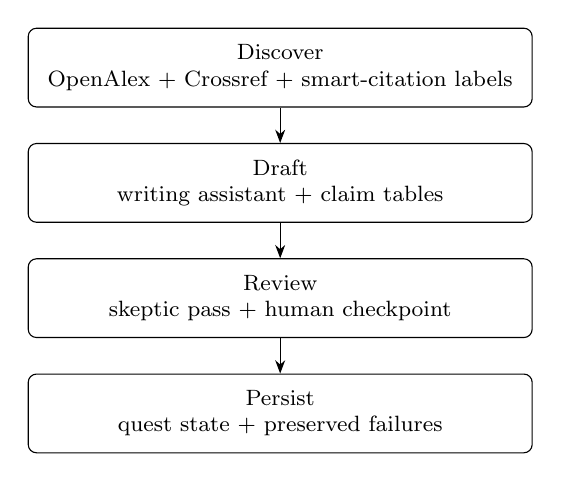
\begin{tikzpicture}[
  font=\footnotesize,
  box/.style={draw, rounded corners=3pt, align=center, minimum width=6.4cm, minimum height=1.0cm},
  >=Stealth
]
\node[box] (a) {Discover\\OpenAlex + Crossref + smart-citation labels};
\node[box, below=0.45cm of a] (b) {Draft\\writing assistant + claim tables};
\node[box, below=0.45cm of b] (c) {Review\\skeptic pass + human checkpoint};
\node[box, below=0.45cm of c] (d) {Persist\\quest state + preserved failures};
\draw[->] (a) -- (b);
\draw[->] (b) -- (c);
\draw[->] (c) -- (d);
\end{tikzpicture}
\caption{Illustrative composite pipeline assembled from the reviewed capabilities.}
\end{figure}

\section{What the Composite Does Not Prove}
Table~5.1 audits each stage against the six success criteria of Chapter~2.
The table records what was and was not evidenced in the reviewed material;
it is not a claim that the products have no additional integrations or
capabilities. The key gap for ResearchX is integration: the target contract
requires the stages to share identifiers, provenance and a human gate.

\begin{table}[ht]
\centering
\caption{Reviewed capability stages and the remaining ResearchX gap}
\small
\begin{tabular}{@{}L{2.7cm}L{3.2cm}L{4.2cm}L{4.1cm}@{}}
\toprule
Stage & Provides & Not evidenced here & ResearchX gap \\
\midrule
Claim mapping & Tables and reports & Shared run ledger & Link to local provenance \\
Draft help & Source-linked writing & Deterministic checks & Preserve evidence IDs \\
Citation context & Support/contrast signals & Experiment linkage & Keep as context, not proof \\
Skeptic pass & Claim review & Human decision record & Connect to checkpoint \\
Quest state & Durable workspace & Cross-source verdicts & Join state to citations \\
\bottomrule
\end{tabular}
\end{table}

% ---------------- Chapter 6 ----------------
\chapter{SOURCE STACK AND VERIFICATION LIMITS}

The intended discovery baseline is independent of any single Scholar-class
service. OpenAlex, Crossref, arXiv and Europe PMC/PubMed cover complementary
metadata, graph, preprint and biomedical/full-text needs; alphaXiv and Pi web
search provide additional discovery surfaces. Table~6.1 separates those
discovery roles from the current citation-verification implementation.

\begin{table}[ht]
\centering
\caption{Discovery and verification sources in the proposed design}
\small
\begin{tabular}{@{}L{2.4cm}L{4.1cm}L{5.7cm}@{}}
\toprule
Function & Source or path & Role and limitation \\
\midrule
Ranking + graph & OpenAlex Works API & Works, citations, topics and OA metadata \\
DOI record & Crossref REST API & Deposited DOI metadata; not claim truth \\
Preprints & arXiv API & Public e-print metadata and identifiers \\
Biomedical text & Europe PMC + PubMed & Search and OA full-text routes \\
Discovery & alphaXiv + Pi web search & Additional retrieval surfaces \\
Verdicts & Current Crossref + Semantic Scholar tool & Deterministic rules; not Scholar-independent \\
\bottomrule
\end{tabular}
\end{table}

The current citation-integrity module still calls Semantic Scholar alongside
Crossref. OpenAlex is available in the science-database layer but is not the
provider used by that verifier. Therefore the report can claim an OpenAlex-
centred discovery baseline, but it cannot claim Scholar-independent citation
verification until the code path is removed or explicitly accepted as a
dependency. The Europe PMC full-text route also applies to its Open Access
subset, and arXiv use must follow the service's API terms and acknowledgement
request~\cite{arxiv}.

% ---------------- Chapter 7 ----------------
\chapter{PROPOSED SOLUTION}

\section{Design on the Pi Base}
ResearchX keeps the four layers of Figure~1.1 and runs them on Pi: the
harness owns the loop and the TUI while research workflows arrive as Pi
extensions, tools, prompts and skills. In the checked-out source tree, the
Research layer has PaperRank scoring, source search and code/audit workflows;
the Integrity layer has citation-integrity and human-checkpoint tools; and the
Writing layer has draft and skeptic workflows. The Kaggle tools implement the
push, status and output path described in Figure~7.1. These are verified
source-tree capabilities, not an independent evaluation of research quality.

The Experiment-layer contract remains partial at this audit date. The source
tree does not yet evidence a dedicated hypothesis-branch findings ledger or a
doom-loop detector, and the workbench still contains additional provider
paths beyond the Kaggle/local default policy. The final report must therefore
describe those items as planned integration work. Nothing in the proposed
design requires a second interaction loop or a copied runtime.

Kaggle Kernels are the default experiment backend and the local workspace is
the offline fallback. Authentication is through the Kaggle environment
variables or the standard configuration file. Specifically, use
\texttt{KAGGLE\_USERNAME} and \texttt{KAGGLE\_KEY}, or
\texttt{\textasciitilde/.kaggle/kaggle.json}. The intended loop is autonomous
and command-line driven, as shown in Figure~7.1:
write the
experiment locally under \texttt{outputs/experiments/\textless slug\textgreater/}
with a single entry script plus helpers and a fast local smoke check only;
push with GPU enabled unless the task is trivial and record the kernel slug
and URL; poll the kernel status every ten minutes until a terminal state of
complete, error, cancelled or failed, re-polling on running or queued;
collect outputs into \texttt{outputs/kaggle/\textless slug\textgreater/};
and report the kernel URL, final state, key metrics from logs, artifact
paths and a one-paragraph diagnosis on failure. Monitoring is delegated to a
runner subagent so it survives context pressure, and a single blocking call
covers push with poll with fetch. The planned guards are hypothesis isolation
with one branch and slug per experiment, an append-only findings ledger of
tried/failed-why/metrics, and a doom-loop detector that kills stuck runs and
saves budget. The first of these is a design rule; the ledger and detector
still require implementation and tests in the current checkout.

\begin{figure}[ht]
\centering
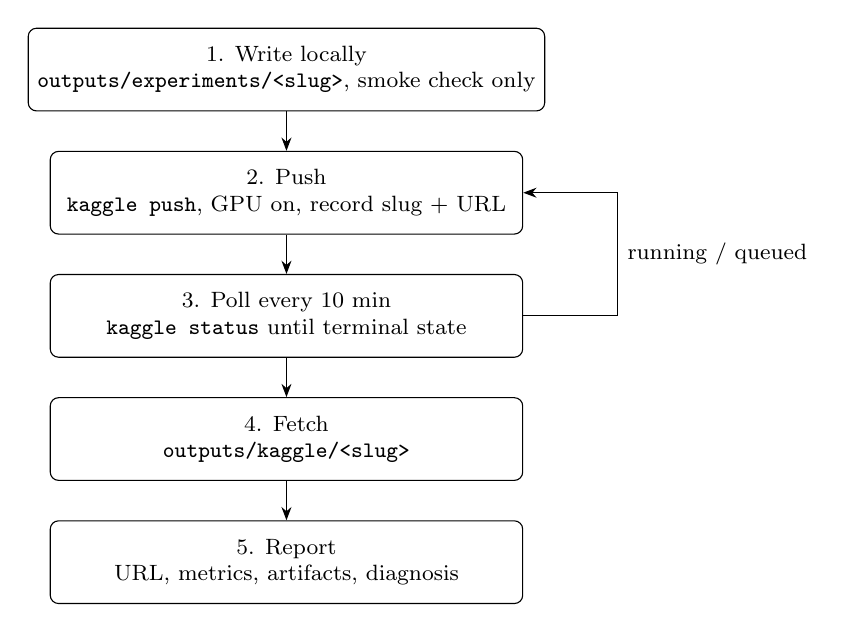
\begin{tikzpicture}[
  font=\footnotesize,
  box/.style={draw, rounded corners=3pt, align=center, minimum width=6cm, minimum height=1.05cm},
  >=Stealth
]
\node[box] (w) {1. Write locally\\\texttt{outputs/experiments/<slug>}, smoke check only};
\node[box, below=0.5cm of w] (p) {2. Push\\\texttt{kaggle push}, GPU on, record slug + URL};
\node[box, below=0.5cm of p] (m) {3. Poll every 10 min\\\texttt{kaggle status} until terminal state};
\node[box, below=0.5cm of m] (f) {4. Fetch\\\texttt{outputs/kaggle/<slug>}};
\node[box, below=0.5cm of f] (r) {5. Report\\URL, metrics, artifacts, diagnosis};
\draw[->] (w) -- (p);
\draw[->] (p) -- (m);
\draw[->] (m) -- (f);
\draw[->] (f) -- (r);
\draw[->] (m.east) -- ++(1.2,0) |- (p.east) node[pos=0.25, right] {running / queued};
\end{tikzpicture}
\caption{Autonomous Kaggle experiment loop with ten-minute monitoring to a
terminal kernel state.}
\end{figure}

\section{Why This Approach Is a Coherent Integration}
The claim is not that ResearchX invents ranking, drafting help, notebook
execution, citation context or skeptic review. Those capabilities already
exist in different products. The proposed contribution is their integration
around a shared artifact and approval contract: the agent can discover
sources, write or push an experiment, collect outputs, attach provenance and
route a draft through citation checks and a human gate. Table~7.1 compares
that target contract with the capabilities evidenced in this review. It is a
design claim, not a completed novelty or superiority result. The current
checkout is not yet entitled to claim the full contract because the citation
provider boundary and experiment ledger/guard work remain incomplete.

\begin{table}[ht]
\centering
\caption{Target ResearchX contract against reviewed capability classes}
\begin{tabular}{@{}L{3.1cm}L{3.1cm}L{4.0cm}L{3.4cm}@{}}
\toprule
Approach & Strength & Missing from the reviewed evidence & ResearchX target \\
\midrule
General chatbots & Flexible generation & Shared evidence record & Source-backed artifacts \\
Literature products & Search, reports, writing & Project-local gate/ledger varies & Integrate with provenance \\
Notebook agents & Runnable, branched experiments & Citation contract varies & Link runs to claims \\
Citation-context tools & Supporting or contrasting signals & Experiment linkage & Treat as context, not proof \\
ResearchX checkout & Pi workflows, Kaggle tools, checkpoint & Verifier/ledger guards partial & Complete and test the contract \\
\bottomrule
\end{tabular}
\end{table}

% ---------------- Chapter 8 ----------------
\chapter{CONCLUSION AND NEXT WORK}

ResearchX currently has a credible Pi-native foundation and several working
research tools, but this audit does not support a claim of a finished,
fully autonomous research system. The highest-priority work is to resolve
the citation-provider policy, implement and test the hypothesis findings
ledger and doom-loop guard, and decide whether the remaining workbench
provider paths are in or out of scope. After that, pin environment
fingerprints for remote runs and evaluate the broad connector registry
against the OpenAlex/Crossref baseline. A human approval remains the final
gate throughout.

All web sources below were accessed on 5 September 2026.

\begin{thebibliography}{15}
\small
\raggedright
\bibitem{pi} Earendil Works. Pi agent harness: \texttt{pi-agent-core}, \texttt{pi-coding-agent}, \texttt{pi-ai} and \texttt{pi-tui}. Agent loop, tool calling, state management, model routing and terminal UI. \url{https://github.com/earendil-works/pi}.
\bibitem{ars} Imbad0202. Academic Research Skills: research, writing, review and stage-gate workflows. \url{https://github.com/imbad0202/academic-research-skills}.
\bibitem{deepscientist} ResearAI. DeepScientist: local-first research studio with quest state, research maps, branches and durable artifacts. \url{https://github.com/ResearAI/DeepScientist}.
\bibitem{elicit} Elicit. AI research agent, paper search, reports, data extraction and cited artifacts. \url{https://elicit.com}.
\bibitem{jenni} Jenni AI. AI academic writing, source-linked suggestions, citation formatting and review features. \url{https://jenni.ai}.
\bibitem{clusy} Clusy. AI IDE for Jupyter notebooks with agent-authored experiments, branching and cloud compute. \url{https://www.clusy.io}.
\bibitem{scite} Scite. AI research platform and Smart Citations for supporting, contrasting and discussing evidence. \url{https://scite.ai}.
\bibitem{openalex} OpenAlex. Works API documentation: scholarly works, citations, topics, open access and query/filter support. \url{https://help.openalex.org/data/works/}.
\bibitem{crossref} Crossref. REST API documentation: public scholarly metadata retrieval, DOI records and query endpoints. \url{https://www.crossref.org/documentation/retrieve-metadata/rest-api/}.
\bibitem{arxiv} arXiv. API access and interoperability guidance. \url{https://info.arxiv.org/help/api/index.html}.
\bibitem{europepmc} Europe PMC. RESTful Web Service: search, citations, references, cross-references and Open Access full-text XML. \url{https://europepmc.org/RestfulWebService}.
\bibitem{alphaxiv} alphaXiv. Paper discovery and analysis surface used by the ResearchX workflow. \url{https://alphaxiv.org}.
\bibitem{kaggle} Kaggle. Official Kaggle CLI: kernel push, status, run, download and output commands. \url{https://github.com/Kaggle/kaggle-cli}.
\bibitem{s2} Semantic Scholar. Academic Graph API referenced by the current citation-integrity implementation. \url{https://api.semanticscholar.org/api-docs/}.
\end{thebibliography}

\end{document}
